\documentclass{report}

\input{preamble}
\input{macros}
\input{letterfonts}

\usepackage{tikz}
\usepackage{tikz-3dplot}
\usepackage{amsmath}
\usepackage{pgfplots}
\usepackage{smartdiagram}
\usesmartdiagramlibrary{additions}
\usepackage{xcolor}
\usepackage{forest}
\usetikzlibrary{circuits.logic.US} % Load the correct library for US-style logic gates
\usepgfplotslibrary{colormaps}
\usepgfplotslibrary{groupplots}
\usepgfplotslibrary{polar}
\pgfplotsset{compat=newest}
\tikzset{>=latex}
\usepackage{siunitx}

\title{\Huge{Intro to Software Engineering}\\EK327}
\author{\huge{Giacomo Cappelletto}}
\date{21/1/25}

\begin{document}


\maketitle
\newpage
\pdfbookmark[section]{\contentsname}{toc}
\tableofcontents
\pagebreak

\chapter{Computer Architecture}

\section{Adding Two Single-Bit Binaries Using XOR and AND Gates}

To add two single-bit binary numbers \( A \) and \( B \), we need to calculate:
1. The \textbf{sum bit}, which is the XOR of \( A \) and \( B \).
2. The \textbf{carry bit}, which is the AND of \( A \) and \( B \).

\textbf{Logic}
- \textbf{Sum Bit:} \( \text{Sum} = A \oplus B \)
- \textbf{Carry Bit:} \( \text{Carry} = A \cdot B \)

\bigskip

The following truth table summarizes the operation:

\[
	\begin{array}{|c|c|c|c|}
		\hline
		A & B & \text{Sum} & \text{Carry} \\
		\hline
		0 & 0 & 0          & 0            \\
		0 & 1 & 1          & 0            \\
		1 & 0 & 1          & 0            \\
		1 & 1 & 0          & 1            \\
		\hline
	\end{array}
\]

\bigskip

The addition is implemented using XOR and AND gates as shown below:

\begin{center}
	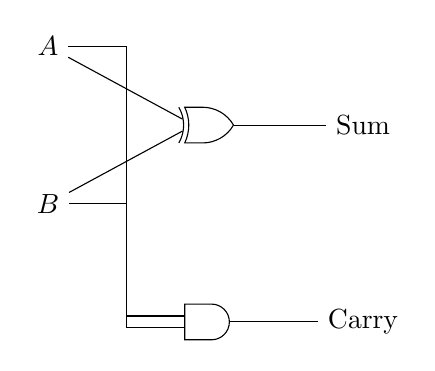
\begin{tikzpicture}[circuit logic US, scale=1, transform shape]

		% Inputs
		\node (A) at (0, 2) {\( A \)};
		\node (B) at (0, 0) {\( B \)};

		% XOR gate
		\node [xor gate US, draw, logic gate inputs=nn] (xor1) at (2, 1) {};
		\draw (A) -- (xor1.input 1);
		\draw (B) -- (xor1.input 2);

		% AND gate
		\node [and gate US, draw, logic gate inputs=nn] (and1) at (2, -1.5) {};
		\draw (A) -- ++(1,0) |- (and1.input 1);
		\draw (B) -- ++(1,0) |- (and1.input 2);

		% Outputs
		\node (Sum) at (4, 1) {\( \text{Sum} \)};
		\node (Carry) at (4, -1.5) {\( \text{Carry} \)};
		\draw (xor1.output) -- (Sum);
		\draw (and1.output) -- (Carry);

	\end{tikzpicture}
\end{center}

The XOR gate produces the sum bit, while the AND gate produces the carry bit. This forms the fundamental building block of a full binary adder.

\section{Adding Two Single-Byte Binary Numbers Using XOR and AND}

Binary addition can be performed on two single-byte numbers using bitwise operations. Specifically:
- The \textbf{XOR (Exclusive OR)} operation gives the sum of two bits without considering the carry.
- The \textbf{AND} operation identifies where a carry will occur.
- The carry is then shifted left by one position and added to the result in subsequent iterations.

\textbf{Algorithm:}
1. Compute the sum without carry using XOR:
   \[
   \text{sum} = a \oplus b
   \]
2. Compute the carry using AND and shift it left by one bit:
   \[
   \text{carry} = (a \land b) \ll 1
   \]
3. Repeat the process by adding the carry to the sum until there is no carry left.

\textbf{Diagram:}
Below is a diagram that illustrates the process for a single bit addition.

\begin{center}
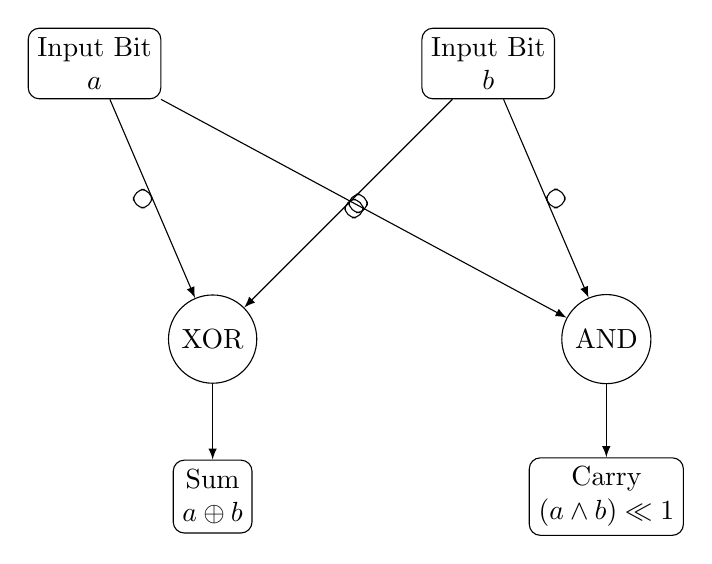
\begin{tikzpicture}[node distance=2cm, every node/.style={draw, rectangle, rounded corners, align=center}]
    % Nodes
    \node (A) {Input Bit \\ $a$};
    \node (B) [right of=A, xshift=3cm] {Input Bit \\ $b$};
    \node (XOR) [below of=A, yshift=-1.5cm, xshift=1.5cm, draw, circle] {XOR};
    \node (SUM) [below of=XOR] {Sum \\ $a \oplus b$};
    \node (AND) [right of=XOR, xshift=3cm, draw, circle] {AND};
    \node (CARRY) [below of=AND] {Carry \\ $(a \land b) \ll 1$};

    % Arrows
    \draw[->] (A) -- (XOR) node[midway, left] {};
    \draw[->] (B) -- (XOR) node[midway, right] {};
    \draw[->] (XOR) -- (SUM);
    \draw[->] (A) -- (AND) node[midway, left] {};
    \draw[->] (B) -- (AND) node[midway, right] {};
    \draw[->] (AND) -- (CARRY);
\end{tikzpicture}
\end{center}

\textbf{Example:}
Consider two single-byte binary numbers:
\[
a = 01101101, \quad b = 10101001
\]

1. Compute the XOR for the sum:
   \[
   \text{sum} = a \oplus b = 11000100
   \]

2. Compute the AND for the carry and shift left:
   \[
   \text{carry} = (a \land b) \ll 1 = 00001010
   \]

3. Add the sum and carry:
   - New sum: \( \text{sum} = 11000100 \oplus 00001010 = 11001110 \)
   - New carry: \( \text{carry} = (11000100 \land 00001010) \ll 1 = 00000000 \)

4. Final result: \( 11001110 \).

\section{One's Complement for a Single Byte}

The \textbf{one's complement} of a binary number is obtained by flipping all the bits, changing every \texttt{1} to \texttt{0} and every \texttt{0} to \texttt{1}. This operation is commonly used in binary arithmetic, particularly in representing negative numbers in early computing systems.

\textbf{Steps to Compute One's Complement:}
1. Write down the binary number.
2. Flip all bits:
   - Change each \texttt{0} to \texttt{1}.
   - Change each \texttt{1} to \texttt{0}.

\textbf{Example:}
Consider the binary number \(a = 01101101\).

1. Original binary number:
   \[
   a = 01101101
   \]

2. One's complement (flip all bits):
   \[
   \text{one's complement of } a = 10010010
   \]

\textbf{Diagram:}
The following diagram illustrates the transformation:

\begin{center}
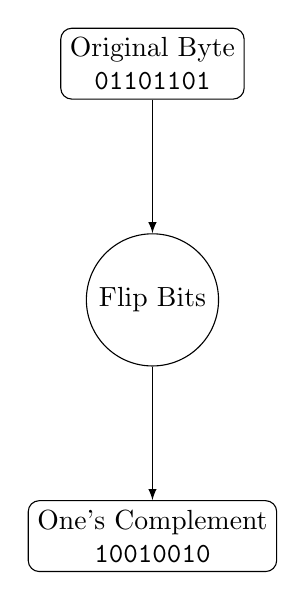
\begin{tikzpicture}[
    node distance=2cm,
    every node/.style={draw, rectangle, rounded corners, align=center}
]
    % Nodes
    \node (Original) {Original Byte \\ \texttt{01101101}};
    \node (Flip) [below of=Original, yshift=-1cm, draw, circle] {Flip Bits};
    \node (Complement) [below of=Flip, yshift=-1cm] {One's Complement \\ \texttt{10010010}};

    % Arrows
    \draw[->] (Original) -- (Flip);
    \draw[->] (Flip) -- (Complement);
\end{tikzpicture}
\end{center}

\textbf{Properties of One's Complement:}
- A binary number and its one's complement always sum to all \texttt{1}s (i.e., \(11111111\) for a single byte).
- One's complement is useful in representing signed integers:
   - Positive numbers are represented as-is.
   - Negative numbers are represented by the one's complement of their positive counterparts.

\textbf{Example with Signed Integers:}
For a single byte:
1. \(+5\) in binary: \(00000101\)
2. \(-5\) in one's complement: \(11111010\)

\textbf{Verification:}
Adding \(+5\) and \(-5\) in one's complement arithmetic:
\[
00000101 + 11111010 = 11111111 \quad (\text{all bits are 1, representing zero in one's complement arithmetic}).
\]

\section{Carrying When Adding Negatives in One's Complement}

In one's complement representation, negative numbers are represented by flipping all the bits of their positive counterparts. When adding two negative numbers, a carry might be generated, which needs to be added back to the result to obtain the correct answer.

\textbf{Example:} Adding \(-3\) and \(-4\).

1. Represent \(-3\) and \(-4\) in one's complement for a single byte:
   \[
   +3 = 00000011, \quad -3 = \text{one's complement of } +3 = 11111100
   \]
   \[
   +4 = 00000100, \quad -4 = \text{one's complement of } +4 = 11111011
   \]

2. Add the two numbers:
   \[
   \begin{array}{c@{}c@{}c@{}c@{}c@{}c@{}c@{}c@{}c}
       & 1 & 1 & 1 & 1 & 1 & 1 & 0 & 0 \\ 
     + & 1 & 1 & 1 & 1 & 1 & 0 & 1 & 1 \\ \hline
       & 1 & 1 & 1 & 1 & 0 & 1 & 1 & 1 \\ 
   \end{array}
   \]

3. Handle the carry:
   - The result of the addition is \(11110111\), with a carry bit of \(1\).
   - Add the carry back to the least significant bit:
     \[
     11110111 + 1 = 11111000
     \]

4. Final result:
   \[
   11111000 = \text{one's complement of } +7 = -7
   \]

\textbf{Explanation:}
- When the sum generates a carry, it must be added back to the result to comply with one's complement rules.
- The result of \(-3 + -4 = -7\), as expected.

\begin{center}
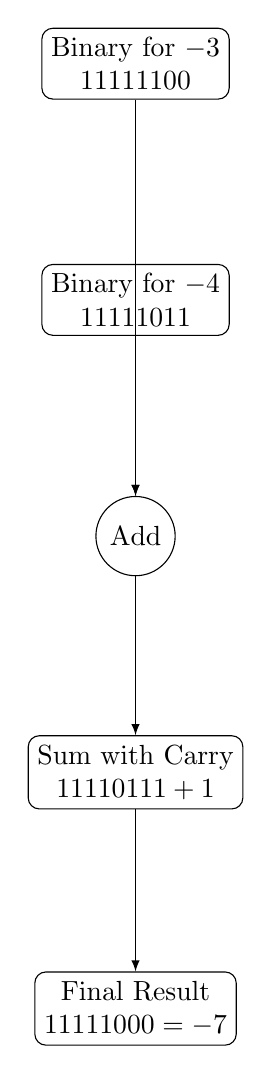
\begin{tikzpicture}[node distance=2cm, every node/.style={draw, rectangle, rounded corners, align=center}]
    % Nodes
    \node (A) {Binary for $-3$ \\ $11111100$};
    \node (B) [below of=A, yshift=-1cm] {Binary for $-4$ \\ $11111011$};
    \node (Add) [below of=B, yshift=-1cm, draw, circle] {Add};
    \node (Sum) [below of=Add, yshift=-1cm] {Sum with Carry \\ $11110111 + 1$};
    \node (Result) [below of=Sum, yshift=-1cm] {Final Result \\ $11111000 = -7$};

    % Arrows
    \draw[->] (A) -- (Add);
    \draw[->] (B) -- (Add);
    \draw[->] (Add) -- (Sum);
    \draw[->] (Sum) -- (Result);
\end{tikzpicture}
\end{center}

\textbf{Note:} This approach works for signed integers in one's complement and highlights the importance of handling the carry bit to ensure accurate results.

\section{Two's Complement for a Single Byte}

The \textbf{two's complement} of a binary number is obtained by flipping all the bits (as in one's complement) and then adding \(1\) to the result. This method is widely used in modern computer systems to represent signed integers.

\textbf{Steps to Compute Two's Complement:}
1. Write down the binary number.
2. Flip all bits (as in one's complement).
3. Add \(1\) to the flipped number.

\textbf{Example:}
Consider the binary number \(a = 01101101\).

1. Original binary number:
   \[
   a = 01101101
   \]

2. Flip all bits (one's complement):
   \[
   10010010
   \]

3. Add \(1\) to the result:
   \[
   \text{two's complement of } a = 10010010 + 1 = 10010011
   \]

\textbf{Diagram:}
The following diagram illustrates the transformation:

\begin{center}
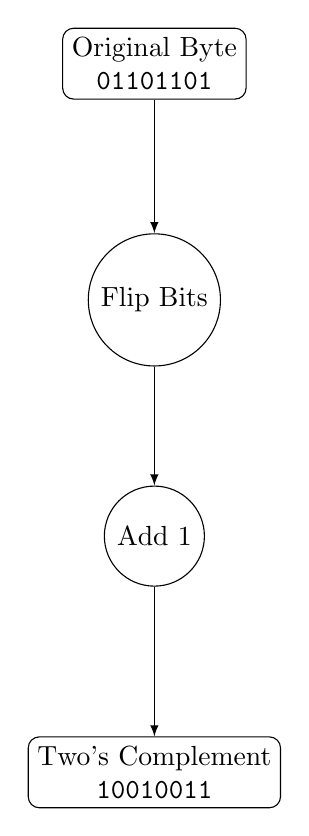
\begin{tikzpicture}[
    node distance=2cm,
    every node/.style={draw, rectangle, rounded corners, align=center}
]
    % Nodes
    \node (Original) {Original Byte \\ \texttt{01101101}};
    \node (Flip) [below of=Original, yshift=-1cm, draw, circle] {Flip Bits};
    \node (Add) [below of=Flip, yshift=-1cm, draw, circle] {Add $1$};
    \node (Complement) [below of=Add, yshift=-1cm] {Two's Complement \\ \texttt{10010011}};

    % Arrows
    \draw[->] (Original) -- (Flip);
    \draw[->] (Flip) -- (Add);
    \draw[->] (Add) -- (Complement);
\end{tikzpicture}
\end{center}

\textbf{Properties of Two's Complement:}
- The two's complement of \(0\) is \(0\), and the two's complement of the maximum negative value is itself.
- Negative numbers are represented by their two's complement.
- Addition and subtraction with two's complement do not require separate subtraction logic, simplifying arithmetic operations.

\section{Carrying When Adding Negatives in Two's Complement}

In two's complement representation, negative numbers are represented by flipping all bits of the positive number and adding \(1\). When adding two negative numbers, the carry generated during addition is discarded.

\textbf{Example:} Adding \(-3\) and \(-4\).

1. Represent \(-3\) and \(-4\) in two's complement for a single byte:
   \[
   +3 = 00000011, \quad -3 = \text{two's complement of } +3 = 11111101
   \]
   \[
   +4 = 00000100, \quad -4 = \text{two's complement of } +4 = 11111100
   \]

2. Add the two numbers:
   \[
   \begin{array}{c@{}c@{}c@{}c@{}c@{}c@{}c@{}c@{}c}
       & 1 & 1 & 1 & 1 & 1 & 1 & 1 & 0 \\ 
     + & 1 & 1 & 1 & 1 & 1 & 1 & 0 & 0 \\ \hline
       & 1 & 1 & 1 & 1 & 1 & 0 & 1 & 1 \\ 
   \end{array}
   \]

3. Handle the carry:
   - The result of the addition is \(11111011\).
   - In two's complement, the carry is ignored, so the final result is:
     \[
     11111011 = -7
     \]

\textbf{Explanation:}
- In two's complement, the carry bit is discarded, unlike in one's complement.
- The result of \(-3 + -4 = -7\), as expected.

\begin{center}
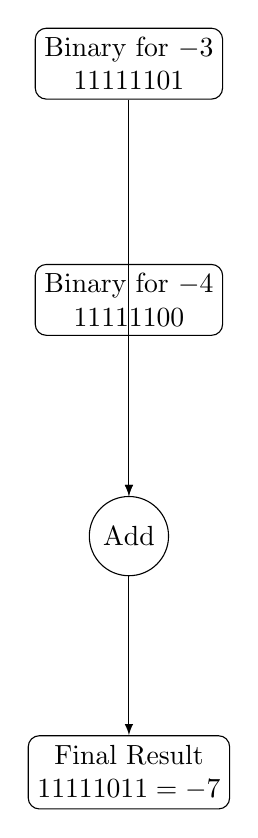
\begin{tikzpicture}[node distance=2cm, every node/.style={draw, rectangle, rounded corners, align=center}]
    % Nodes
    \node (A) {Binary for $-3$ \\ $11111101$};
    \node (B) [below of=A, yshift=-1cm] {Binary for $-4$ \\ $11111100$};
    \node (Add) [below of=B, yshift=-1cm, draw, circle] {Add};
    \node (Result) [below of=Add, yshift=-1cm] {Final Result \\ $11111011 = -7$};

    % Arrows
    \draw[->] (A) -- (Add);
    \draw[->] (B) -- (Add);
    \draw[->] (Add) -- (Result);
\end{tikzpicture}
\end{center}

\textbf{Note:} Two's complement simplifies arithmetic operations by eliminating the need to add back the carry. It is the most commonly used method for representing signed integers in modern computing systems.

\end{document}
